\documentclass[utf8]{book}

\usepackage{ctex}

% syntonly可以在导言区使用\syntaxonly命令,只排错,不生成DVI或PDF文档
\usepackage{syntonly}
% 如果需要生存文档,请将下一行注释掉
% \syntaxonly

\usepackage{verbatim}
\usepackage{fancyvrb}
\usepackage{listings}
\usepackage{graphicx}

\graphicspath{{figures/}}

\usepackage{subfig}
\usepackage{amsmath}
\usepackage{amsfonts}
\usepackage{amssymb}
\usepackage{amsthm}
\usepackage{natbib}
\usepackage{color}
\usepackage{xcolor}
\usepackage{tikz}

% hyperref将很多东西都封装成链接,易与其他包冲突,一般放在最后。
\usepackage{hyperref}

\usepackage{makeidx}
\makeindex

\newcommand{\latexcommand}[1]{\fbox{\textbf{\textbackslash #1}}}
\newcommand{\latexpackage}[1]{\fcolorbox{blue}{yellow}{\textbf{\underline{#1}}}}

\newtheorem{mathdefintion}{定义}[section]


\title{\LaTeX 学习笔记}
\author{Roger Young\thanks{Email: rogeryoung@outlook.com}}
\date{\today}

\begin{document}
	\maketitle
	
	\frontmatter
	
	\tableofcontents
	
	\mainmatter
	
	\chapter{基础知识}
	\section{编码实践}
	中文编码将以使用ctex宏包,文档类使用UTF-8编码,并且使用xelatex命令编译。
	\section{\LaTeX 中的字符}
	\LaTeX 文档源代码中,\textbf{空格键}和\textbf{Tab键}输入的空白字符被视为“空格”。连续的多个空白字符被视为一个空格。每一行开头的空格忽略不计。
	
	行末的回车视为一个空格,所导致的效果一般是换行,但不分段。连续的两个回车,也就是空行,会将文字分段。多个连续的(或者以空白字符分隔的)空行会被认为是一个空行。也可以在行末使用命令\latexcommand{par} 强制分段。
	
	\LaTeX 原文档使用“\%”字符来表示注释。在这个字符到其后第一个回车符之前的字符都将被忽略。
	
	\subsection{\LaTeX 的特殊字符的输入}
	\begin{tabular}{|c|c|c|}
		\hline
		特殊字符 & \LaTeX 中特殊意义 & 输入方式 \\
		\hline
		\# &  & \\
		\hline
		\$ & 用于排版\textbf{行内}数学公式 & \\
		\hline
		\% & & \\
		\hline
		\& & 用于输入表格,分隔每列 & \\
		\hline
		\{ & & \\
		\hline
		\}& & \\
		\hline
		\_ & 数学公式中用于表示下标 &  \\
		\hline
		\^ & 数学公式中用于表示上标 & \latexcommand{\^} \\
		\hline
		\textbackslash  & 输入特殊字符,输入命令 & \latexcommand{textbackslash} \\
		\hline
		\textbackslash [  & 输入公式块 & \latexcommand{textbackslash} [ \\
		\hline
	\end{tabular}
	
	\subsection{特殊标点符号的输入}
		\LaTeX 中有三种长度的“横线”可以使用:连字号(-)、短破折号(--)和长破折号(---)。连字号主要用来组成复合词(father-in-law)、短破折号用来表示数字范围(2007--2011 )、长破折号作为破折号使用(Yes---or No?)。
	
		省略号(\ldots)的输入可以采用命令\latexcommand{ldots}、\latexcommand{dots},这两个命令等价。
	
		波浪号有两种:其中“\~ ”可以使用命令“\latexcommand{textbackslash}\~”输入,$ \sim $ 可以使用\latexcommand{sim}输入。
		
	\subsection{文本强调}\label{text_emphasis}
		强调文本的方式有很多中,比如可以采用\underline{下划线},可以采用\textit{斜体},或者\textbf{加粗}。\underline{对于比较长的部分采用默认的下划线容易引起一些问题,比如无法换行,blalalalalalala},不同的单词可能产生不同高低的下划线。这种情况可以借用\latexpackage{ulem}包来解决,可以采用\latexcommand{uline}轻松生成自动换行的下划线。
		
	\section{交叉引用和脚注}
		引用是\LaTeX 很强大的功能之一。在可以交叉引用的地方,可以使用\latexcommand{label}命令。然后在其他地方通过命令\latexcommand{ref}和\latexcommand{pageref}来引用。有关文本强调的备份,请参考第\pageref{text_emphasis}页\ref{text_emphasis},访问文本强调部分。而制作脚注,可以参考脚注\footnote{直接在文中插入\latexcommand{footnote}即可。}。而对于某些不能正确生成脚注的地方,比如表格环境,可以先在需要插入脚注的地方,使用命令\latexcommand{footnotemark}为脚注计数,然后再在合适的位置用命令\latexcommand{footnotetext}生成脚注。
		
		\begin{tabular}{l}
			\hline
			“天地玄黄,宇宙洪荒。日月盈昃,辰宿列张。”\footnotemark \\
			\hline
		\end{tabular}
		\footnotetext{表格里的名句出自《千字文》。}
		
	\section{特殊环境}
		\subsection{引用环境}
		\latexcommand{quote}用于引用较短的文字,首行不缩进。
		\begin{quote}
			冯唐易老,李广难封。屈贾谊于长沙,非无圣主;窜梁鸿于海曲,岂乏明时?所赖君子见机,达人知命。老当益壮,宁移白首之心?穷且益坚,不坠青云之志。酌贪泉而觉爽,处涸辙以犹欢。
		\end{quote}
	
		\latexcommand{verse}适用于诗歌排版,首行悬挂缩进。
		\begin{verse}
			噫吁嚱,危乎高哉!
			蜀道之难,难于上青天!
			蚕丛及鱼凫,开国何茫然!
			尔来四万八千岁,不与秦塞通人烟。
			西当太白有鸟道,可以横绝峨嵋巅。
			地崩山摧壮士死,然后天梯石栈方钩连。
			上有六龙回日之高标,下有冲波逆折之回川。
			黄鹤之飞尚不得过,猿猱欲度愁攀援。
			青泥何盘盘,百步九折萦岩峦。
			扪参历井仰胁息,以手抚膺坐长叹。
			问君西游何时还?畏途巉岩不可攀。
			但见悲鸟号古木,雄飞从雌绕林间。
			又闻子规啼夜月,愁空山。
			蜀道之难,难于上青天,使人听此凋朱颜。
			连峰去天不盈尺,枯松倒挂倚绝壁。
			飞湍瀑流争喧豗,砯崖转石万壑雷。
			其险也若此,嗟尔远道之人,胡为乎来哉。
			剑阁峥嵘而崔嵬,一夫当关,万夫莫开。
			所守或匪亲,化为狼与豺。
			朝避猛虎,夕避长蛇,
			磨牙吮血,杀人如麻。
			锦城虽云乐,不如早还家。
			蜀道之难,难于上青天,侧身西望长咨嗟。
		\end{verse}
		
		\latexcommand{quotation}适用于打断文字,并且进行首行缩进。
		逍遥游:
		\begin{quotation}
			北冥有鱼,其名为鲲。鲲之大,不知其几千里也;化而为鸟,其名为鹏。鹏之背,不知其几千里也;怒而飞,其翼若垂天之云。是鸟也,海运则将徙于南冥。南冥者,天池也。
			《齐谐》者,志怪者也。《谐》之言曰:“鹏之徙于南冥也,水击三千里,抟扶摇而上者九万里,去以六月息者也。”野马也搜索,尘埃也,生物之以息相吹也。天之苍苍,其正色邪?其远而无所至极邪?其视下也,亦若是则已矣。
			且夫水之积也不厚,则其负大舟也无力。覆杯水于坳堂之上,则芥为之舟;置杯焉则胶,水浅而舟大也。风之积也不厚,则其负大翼也无力。故九万里,则风斯在下矣,而后乃今培风;背负青天,而莫之夭阏者,而后乃今将图南。
			蜩与学鸠笑之曰:“我决起而飞,抢榆枋而止,时则不至,而控于地而已矣,奚以之九万里而南为?”适莽苍者,三餐而反,腹犹果然;适百里者,宿舂粮;适千里者,三月聚粮。之二虫又何知!
			小知不及大知,小年不及大年。奚以知其然也?朝菌不知晦朔,蟪蛄不知春秋,此小年也。楚之南有冥灵者,以五百岁为春,五百岁为秋;上古有大椿者,以八千岁为春,八千岁为秋。此大年也。而彭祖乃今以久特闻,众人匹之,不亦悲乎?
			汤之问棘也是已。穷发之北,有冥海者,天池也。有鱼焉,其广数千里,未有知其修者,其名为鲲。有鸟焉,其名为鹏,背若泰山,翼若垂天之云;抟扶摇羊角而上者九万里,绝云气,负青天,然后图南,且适南冥也。斥鷃笑之曰:“彼且奚适也?我腾跃而上,不过数仞而下,翱翔蓬蒿之间,此亦飞之至也。而彼且奚适也?”此小大之辩也。
			故夫知效一官、行比一乡、德合一君、而征一国者,其自视也,亦若此矣。而宋荣子犹然笑之。且举世誉之而不加劝,举世非之而不加沮,定乎内外之分,辩乎荣辱之境,斯已矣。彼其于世,未数数然也。虽然,犹有未树也。夫列子御风而行,泠然善也,旬有五日而后反。彼于致福者,未数数然也。此虽免乎行,犹有所待者也。若夫乘天地之正,而御六气之辩,以游无穷者,彼且恶乎待哉?故曰:至人无己,神人无功,圣人无名。
			尧让天下于许由,曰:“日月出矣,而爝火不息;其于光也,不亦难乎?时雨降矣,而犹浸灌;其于泽也,不亦劳乎?夫子立而天下治,而我犹尸之;吾自视缺然,请致天下。”许由曰:“子治天下,天下既已治也;而我犹代子,吾将为名乎?名者,实之宾也;吾将为宾乎?鹪鹩巢于深林,不过一枝;偃鼠饮河,不过满腹。归休乎君,予无所用天下为!庖人虽不治庖,尸祝不越樽俎而代之矣!”
			肩吾问于连叔曰:“吾闻言于接舆,大而无当,往而不反。吾惊怖其言。犹河汉而无极也;大有迳庭,不近人情焉。”连叔曰:“其言谓何哉?”曰:“藐姑射之山,有神人居焉。肌肤若冰雪,淖约若处子,不食五谷,吸风饮露,乘云气,御飞龙,而游乎四海之外;其神凝,使物不疵疠而年谷熟。吾以是狂而不信也。”连叔曰:“然。瞽者无以与乎文章之观,聋者无以与乎钟鼓之声。岂唯形骸有聋盲哉?夫知亦有之!是其言也犹时女也。之人也,之德也,将旁礴万物以为一,世蕲乎乱,孰弊弊焉以天下为事!之人也,物莫之伤:大浸稽天而不溺,大旱金石流,土山焦而不热。是其尘垢秕糠将犹陶铸尧舜者也,孰肯以物为事?”宋人资章甫而适诸越,越人断发文身,无所用之。尧治天下之民,平海内之政,往见四子藐姑射之山,汾水之阳,窅然丧其天下焉。
			惠子谓庄子曰:“魏王贻我大瓠之种,我树之成,而实五石。以盛水浆,其坚不能自举也。剖之以为瓠,则瓠落无所容。非不呺然大也,吾为其无用而掊之。”庄子曰:“夫子固拙于用大矣。宋人有善为不龟手之药者,世世以洴澼絖为事。客闻之,请买其方百金。聚族而谋曰:‘我世世为洴澼絖,不过数金,今一朝而鬻技百金,请与之。’客得之,以说吴王。越有难,吴王使之将,冬,与越人水战,大败越人。裂地而封之。能不龟手一也,或以封,或不免于洴澼絖,则所用之异也。今子有五石之瓠,何不虑以为大樽,而浮于江湖,而忧其瓠落无所容?则夫子犹有蓬之心也夫!”
			惠子谓庄子曰:“吾有大树,人谓之樗。其大本拥肿而不中绳墨,其小枝卷曲而不中规矩,立之涂,匠人不顾。今子之言大而无用,众所同去也。”庄子曰:“子独不见狸狌乎?卑身而伏,以候敖者;东西跳梁,不辟高下;中于机辟,死于罔罟。今夫斄牛,其大若垂天之云。此能为大矣,而不能执鼠。今子有大树,患其无用,何不树之于无何有之乡,广莫之野,彷徨乎无为其侧,逍遥乎寝卧其下。不夭斤斧,物无害者,无所可用,安所困苦哉!”
		\end{quotation}
	\subsection{代码环境}LaTeX
		\begin{verbatim}
#include <iostream>
int main()
{
	std::cout << "Hello, LaTeX" << std::endl;
	return 0;
}
		\end{verbatim}
	
		\subsection{图片}
			下面插入一张图片:
			
			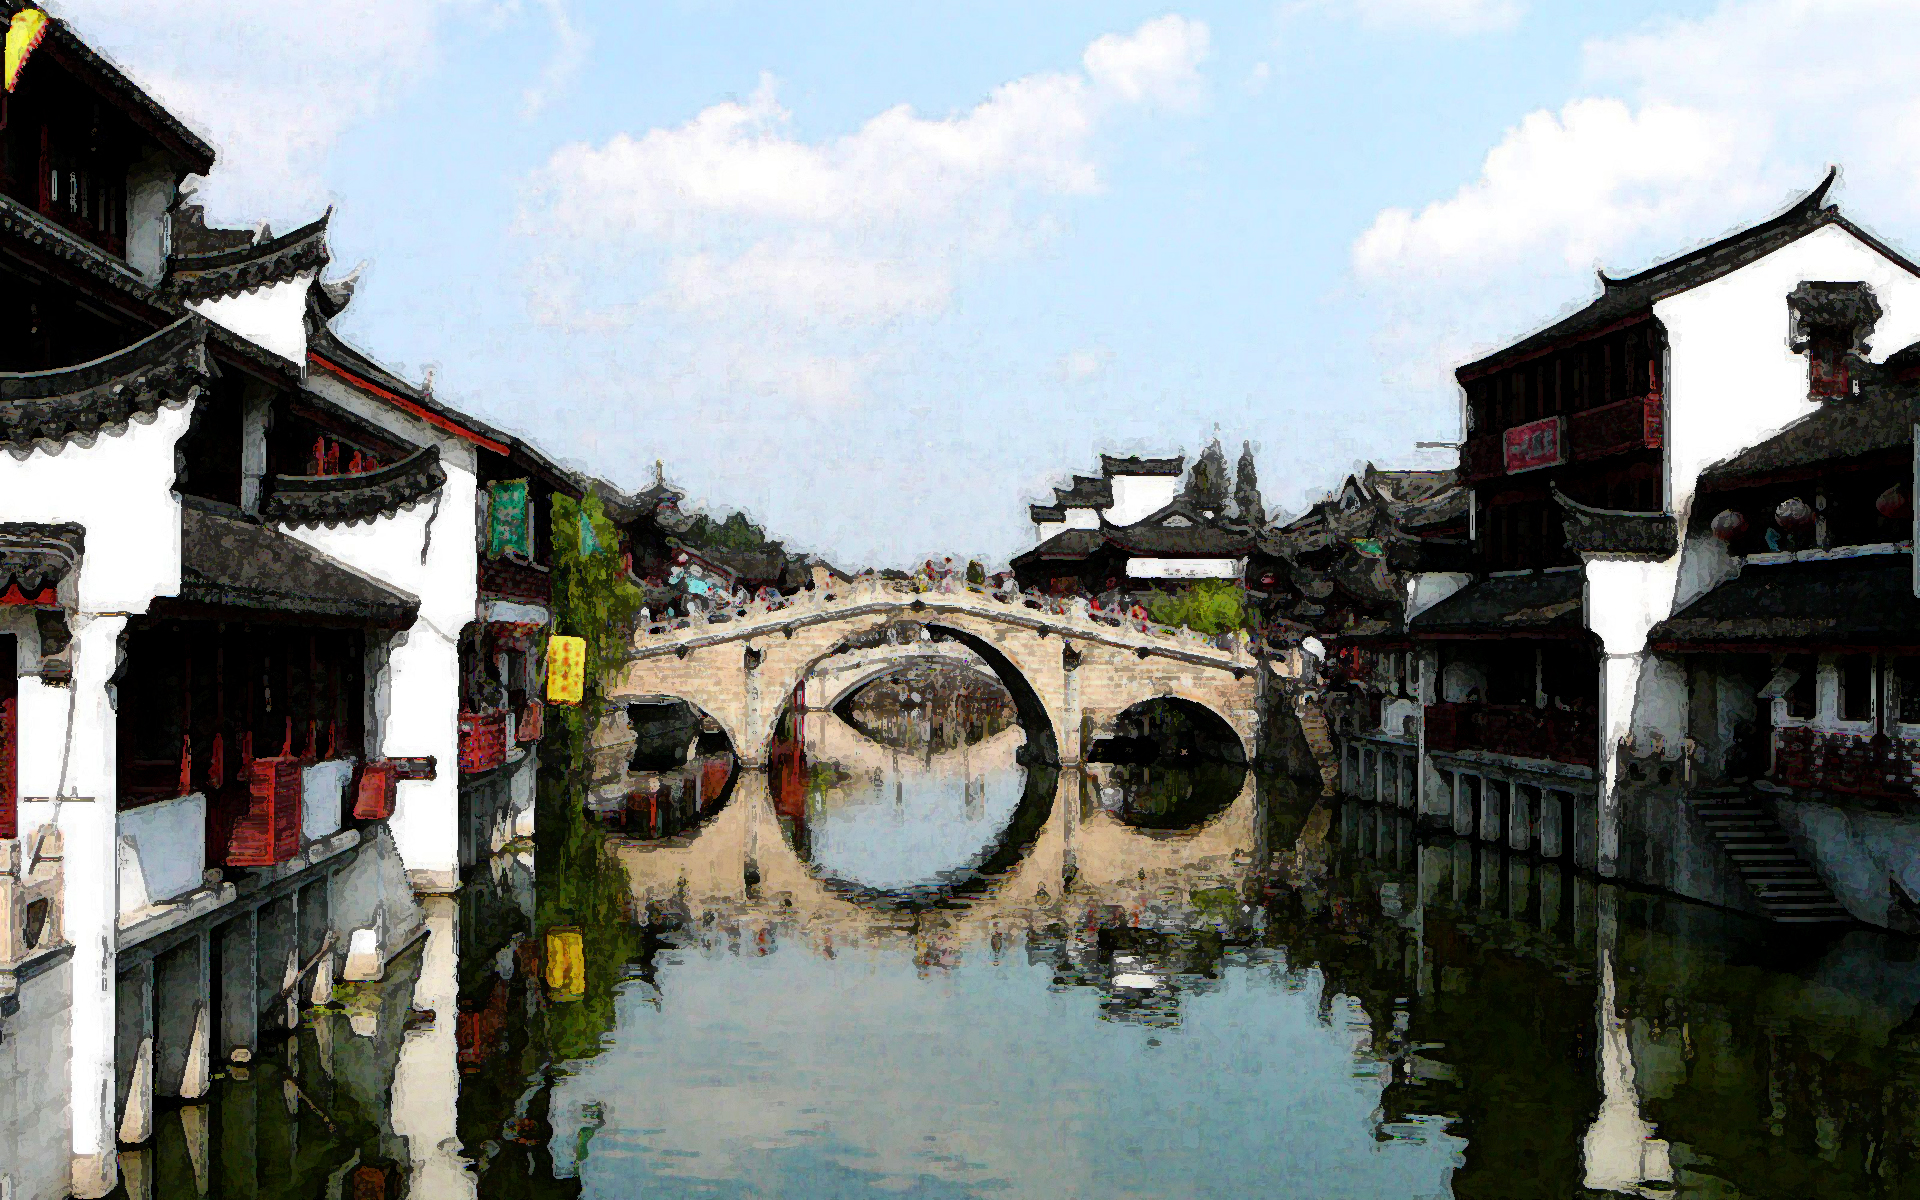
\includegraphics[scale=0.1]{house.jpeg}
			
			\begin{figure}[htbp]
				\centering
				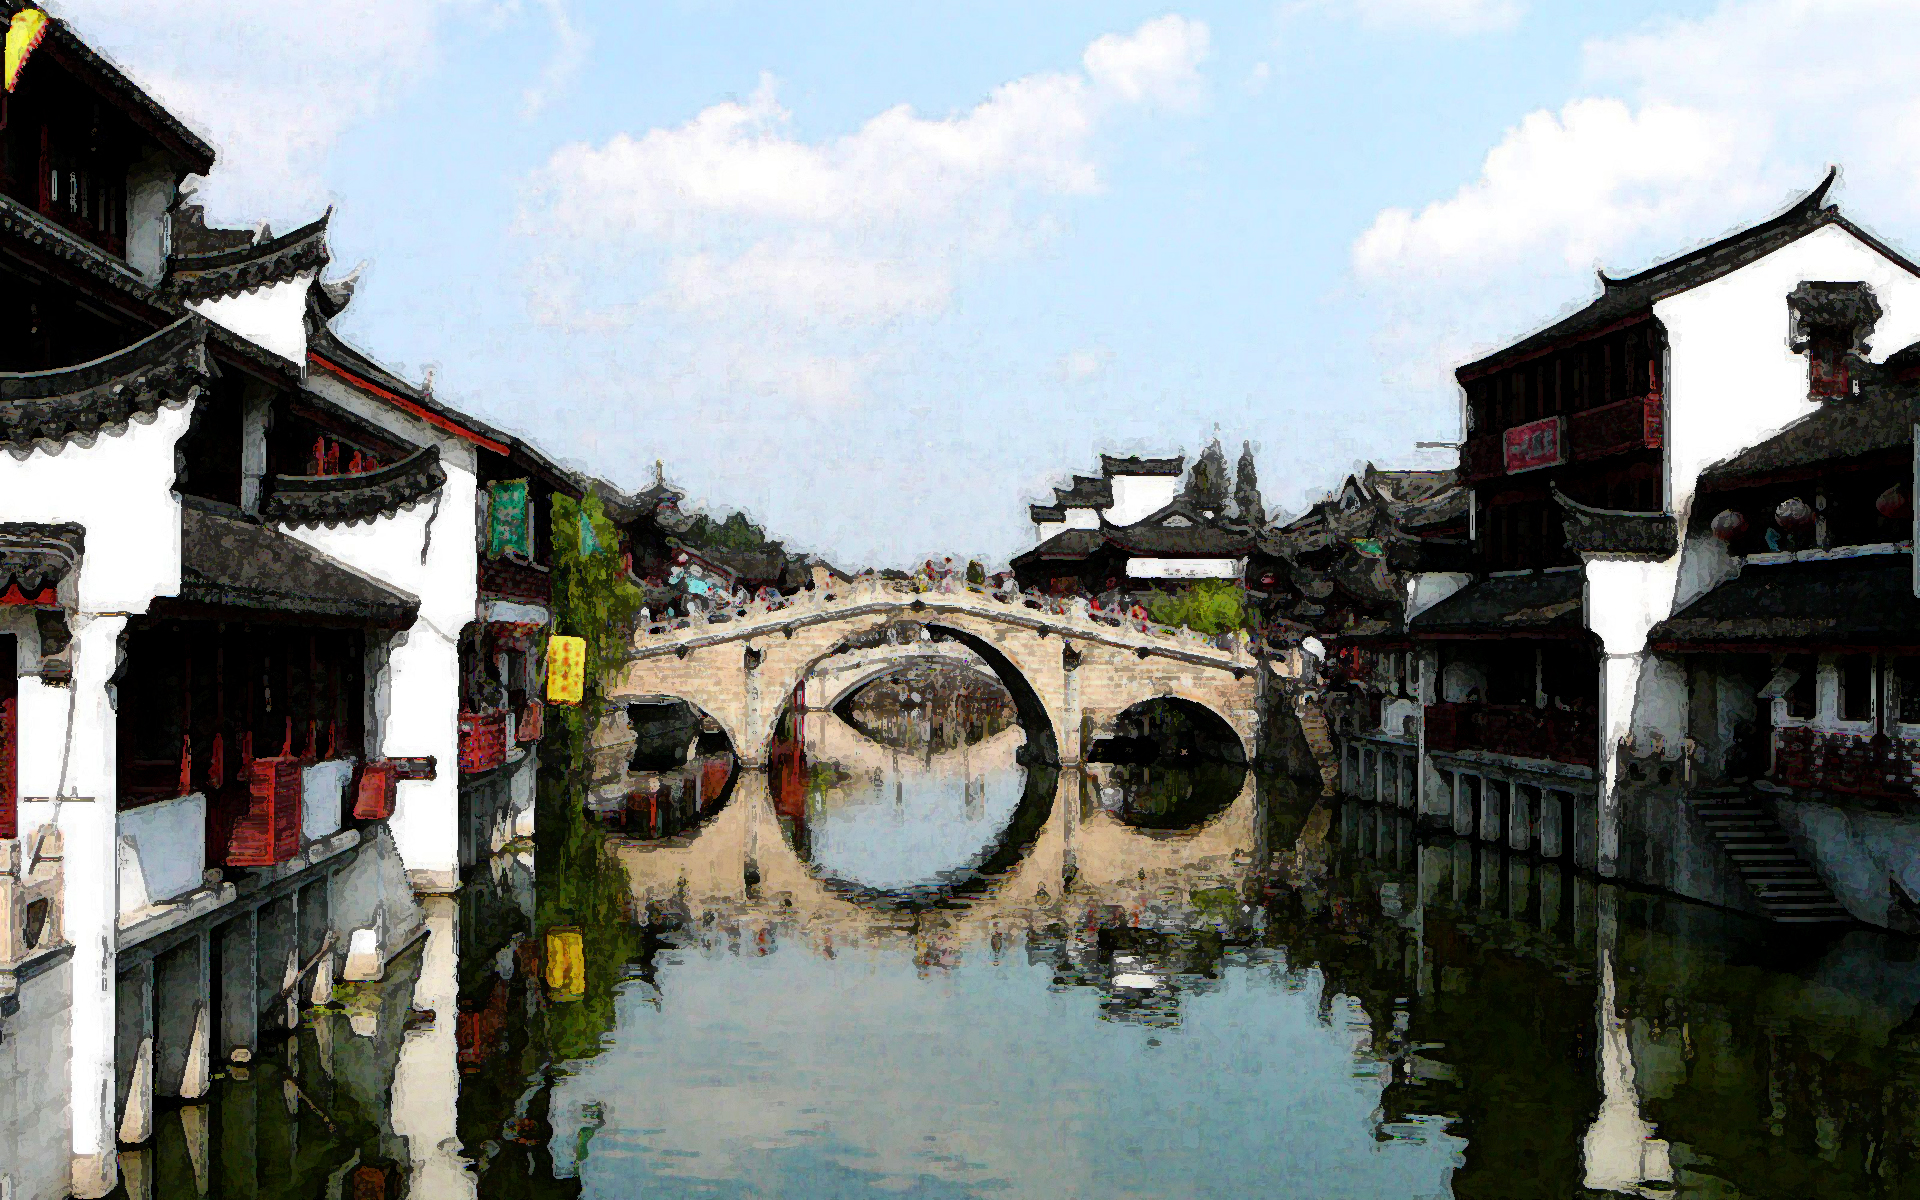
\includegraphics[scale=0.05]{house.jpeg}
				\qquad
				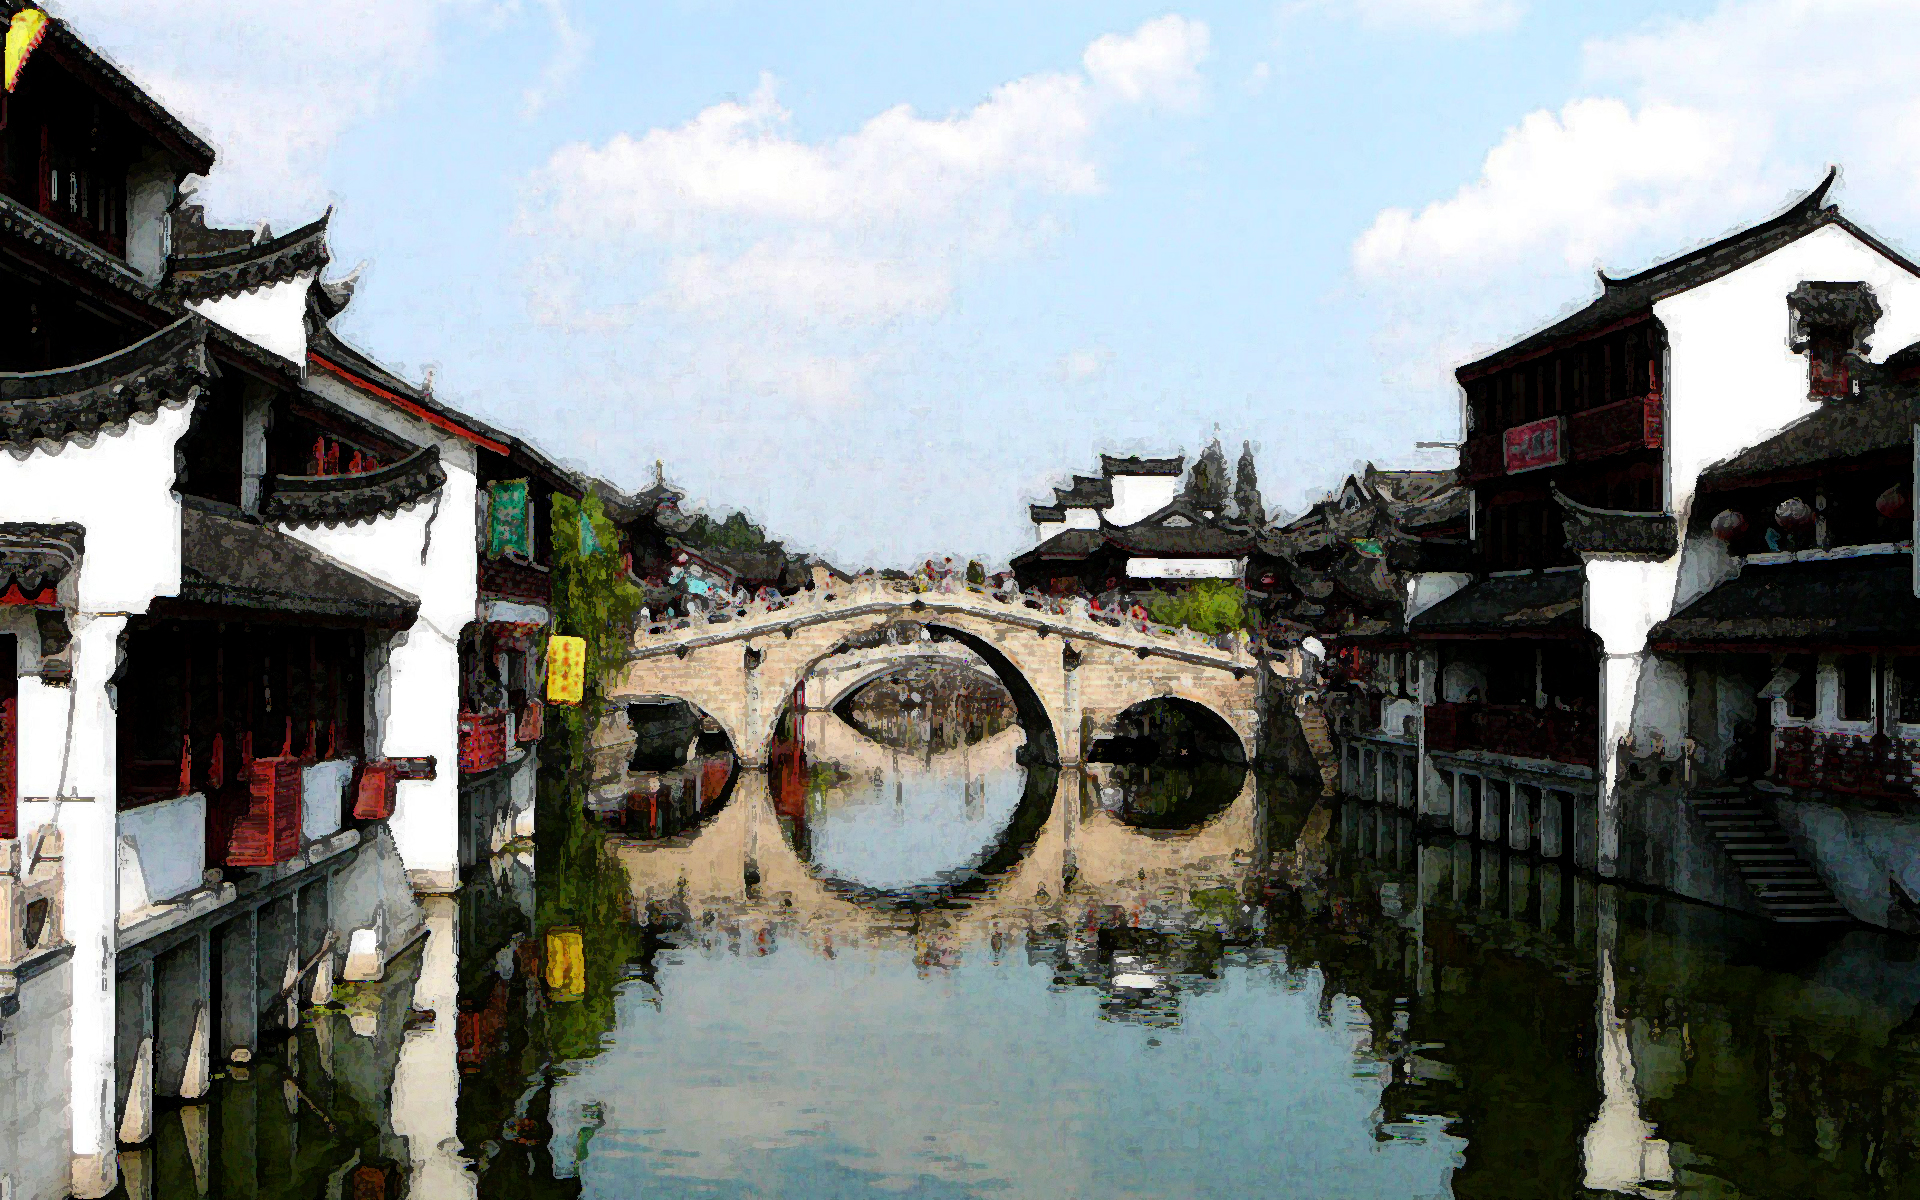
\includegraphics[scale=0.05]{house.jpeg}
				
				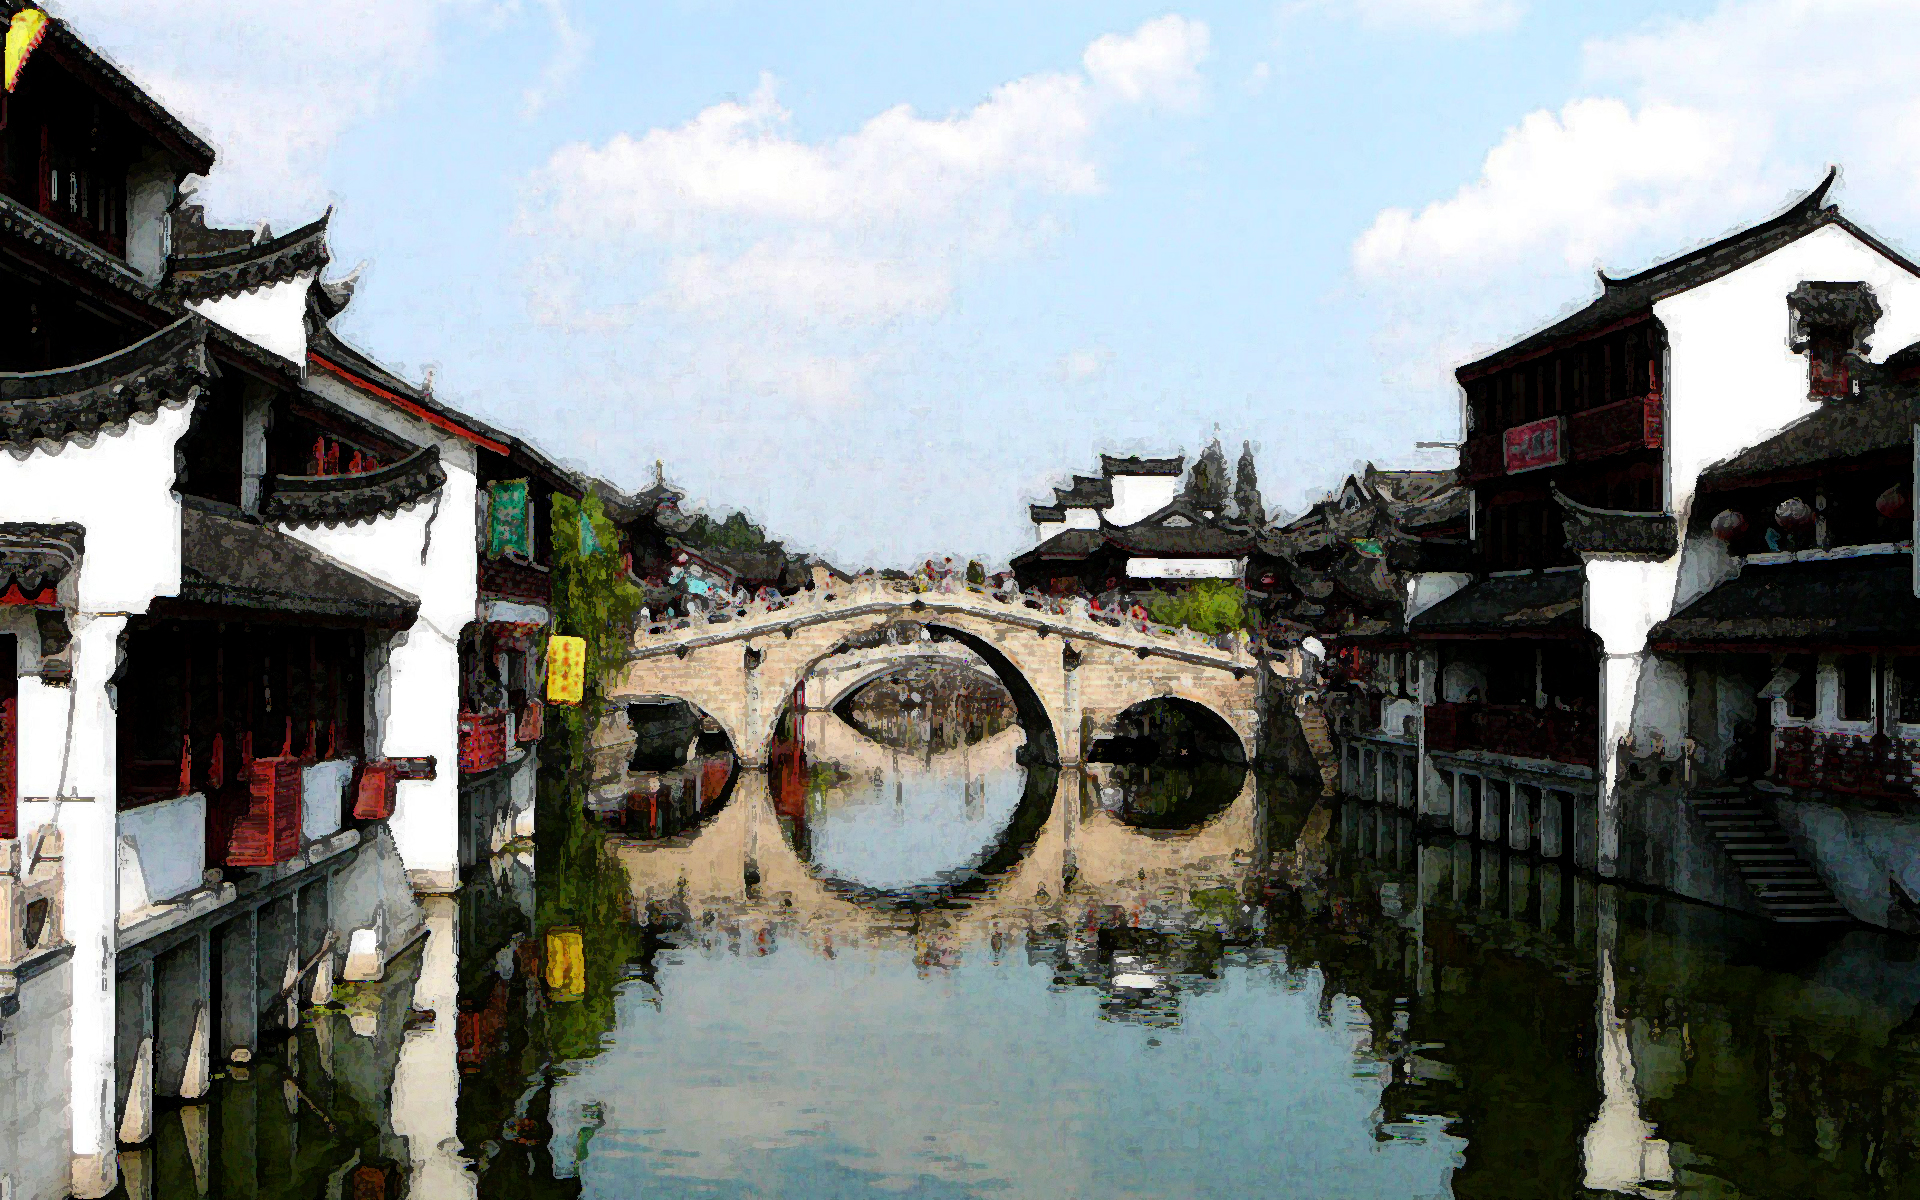
\includegraphics[scale=0.12]{house.jpeg}
				\caption{并排排版图片}
			\end{figure}
			
		\subsection{盒子}
			以下是这一行是\latexcommand{mbox}的示例,可以看到\latexcommand{mbox}会生成一个基本的水平盒子,内容只有一行。也不允许分段。看看会不会换行吧(看看能否看到后面的中文哦)。
			
			\mbox{\footnotemark We the People of the United States, in Order to form a more perfect Union, establish Justice, insure domestic Tranquility, provide for the common defence, promote the general Welfare, and secure the Blessings of Liberty to ourselves and our Posterity, do ordain and establish this Constitution for the United States of America. 不好意思,这里您估计看不到哦}
			\footnotetext{Constitution for the United States of America}
			
			|\makebox[10em]{Test some words.}|\\
			|\makebox[10em][l]{Test some words.}|\\
			|\makebox[10em][r]{Test some words.}|\\
			|\makebox[10em][s]{Test some words.}|
			
			\fbox{老当益壮,宁移白首之心?穷且益坚,不坠青云之志。}
			
			三字经:\parbox[t]{3em}%
			{人之初性本善性相近习相远}
			\quad
			千字文:
			\begin{minipage}[b][8ex][t]{5em}
				天地玄黄
				
				宇宙洪荒\footnote{千字文}
			\end{minipage}
		
			\rule{1em}{1em} Two Black Box \rule{1em}{1em}
			
			We the People \rule[-.4pt]{5em}{.4pt} the United States
			
		\subsection{浮动体}
		
	\section{公式}
		小试牛刀:
		
		$ f(x) = x^2 \quad f'(x) = 2x \quad f''^{2}(x)=4 $
		
		$ p^3_{ij} \qquad m_\mathrm{Knuth}\qquad
		\sum_{k=1}^3 k $
		
		$ a^x+y \neq a^{x+y}\qquad e^{x^2} \neq {e^x}^2 $
		
		分式的输入可以使用\latexcommand{frac}命令,比如$ \frac{x+y}{x-y} $,可以看到,在行内输入分式时,体验很不好。可以采用\latexpackage{amsmath}包内提供的\latexcommand{dfrac}改善一下:$ \dfrac{x+y}{x-y} $。
		
		根式的输入可以采用\latexcommand{sqrt}命令,比如$ \sqrt{x} \Leftrightarrow x^{1/2} $、$ \sqrt[3]{2} $、$ \sqrt{x^{2} + \sqrt{y}} $、$ \sqrt{x^{2} + \sqrt{y + \sqrt{z+10^{\frac{y}{z}}}}} $。
		
		特殊的分式形式,如二项式结构,可以有\latexpackage{amsmath}包内提供的\latexcommand{binom}命令输入:
		\begin{equation}
			\binom{n}{k} =\binom{n-1}{k} + \binom{n-1}{k-1}
		\end{equation}
		
		$ \underline{\underline{\underline{\underline{\underline{\overline{x+y}_0}}}}} $好吓人呀。
		
		$ \underbrace{\overbrace{a+b+c}^{a+\frac{3}{4}} \cdot \overbrace{d+e+f}^7}_\text{meaning of life} = 42 $
		
		一个多行公式:
		\begin{multline}
			a + b + c + d + e + f + g + h + i \\
			= j + k + l + m + n\\
			= o + p + q + r + s\\
			= t + u + v + x + z \qquad
			\rule{1em}{1em} \notag
		\end{multline}
		
		更好的展示形式:
		\begin{align}
			a & = b + c \\
			& = d + e
		\end{align}
		
		\begin{align}
			a & =1 & b &=2 & c &=3 \\
			d &=-1 & e &=-2 & f &=-5
		\end{align}
		
		\begin{gather}
			a = b + c \\
			d = e + f + g \\
			h + i = j + k \notag \\
			l + m = n
		\end{gather}
		
		\begin{equation}
			\begin{aligned}
				a &= b + c \\
				d &= e + f + g \\
				h + i &= j + k \\
				l + m &= ns
			\end{aligned}
		\end{equation}
		
		\begin{equation}
			\mathbf{X} = \left(
			\begin{array}{ccc}
			x_1 & x_2 & \ldots \\
			x_3 & x_4 & \ldots \\
			\vdots & \vdots & \ddots
			\end{array} \right)
		\end{equation}
		
		\begin{equation}
			|x| = \left\{
			\begin{array}{rl}
			-x & \text{if } x < 0,\\
			0 & \text{if } x = 0,\\
			x & \text{if } x > 0.
			\end{array} \right.
		\end{equation}
		
		\begin{equation}
			|x| =
			\begin{cases}
			-x & \text{if } x < 0,\\
			0 & \text{if } x = 0,\\
			x & \text{if } x > 0.
			\end{cases}
		\end{equation}
		
		\begin{mathdefintion}
			$ E = mc^2 $
		\end{mathdefintion}
		
		\section{参考文献}
		\bibliographystyle{plain}
		
		\index{参考文献说明} The cancer epigenome: Concepts, challenges, and therapeutic opportunities \cite{Dawson1147}
		
		
		Partl~\cite{pa} has proposed that \ldots
		
		
	
	\section{颜色}
		\large\sffamily {\color[gray]{0.6} 60\% 灰色} \\
		{\color[rgb]{0,1,1} 青色}
		\label{great_color}
		
	\section{超链接}
		\url{http://wikipedia.org} \\
		\nolinkurl{http://wikipedia.org} \\
		\href{http://wikipedia.org}{Wiki}
		\hyperref[great_color]{维基百科}
	
	\section{绘图}
		绘图示例:
		
		\begin{tikzpicture}
			% 定义点
			\coordinate (ori) at (0,0);
			\coordinate (rect) at (2cm, 2cm);
			% 划直线
			\draw (ori) -- (rect);		
			\draw (5, 0) -- (6,2) --(4,3) -- cycle;
			% 划方形
			\draw (ori) rectangle(2, 1);
			% 划圆
			\draw (ori) circle (2+1);
			% 划椭圆
			\draw (ori) ellipse [x radius=2, y radius=1];
			% 划直角
			\draw (6,0) |- (7,1);
			\draw (-1,-1) -| (-2,-3);
			% 划弧线
			\draw (4,0) arc (0:135:1);
		\end{tikzpicture}
		
		\begin{tikzpicture}
			% 划贝塞尔曲线
			\draw (0,0) .. controls (2,1) and (3,1) .. (3,0);
			\draw (4,0) .. controls (5,1) .. (5,0);
			\draw[help lines] (0,0) -- (2,1) -- (3,1) -- (3,0)
			(4,0) -- (5,1) -- (5,0);
			% 绘制网格
			\draw[help lines,step=0.5] (-2,-2) grid (2,2);
			\draw[->] (-2.5,0) -- (2.5,0);
			\draw[->] (0,-2.5) -- (0,2.5);
			% 绘制函数图形
			\draw[domain=-2:2] plot(\x,{\x*\x*\x});
			\draw[domain=-2:2] plot(\x,{\x*\x-2});
			% 写文字
			\node (A) at (0,0) {A};
			\node (B) at (1,0) {B};
			\node (C) at (60:1) {C};
			\draw (A) -- (B) -- (C) -- (A);
		\end{tikzpicture}
		
		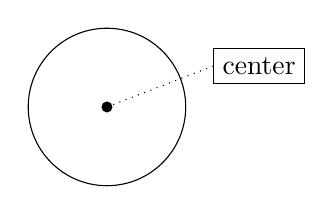
\begin{tikzpicture}
			\draw (0,0) circle[radius=1];
			\fill (0,0) circle[radius=2pt];
			\node[draw] (P) at (15:2) {center};
			\draw[dotted] (0,0) -- (P.west);
		\end{tikzpicture}
		
		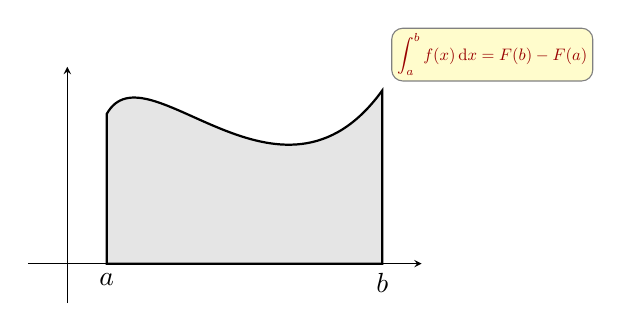
\begin{tikzpicture}
			\draw[-stealth,line width=0.2pt] (-0.5,0) -- (4.5,0);
			\draw[-stealth,line width=0.2pt] (0,-0.5) -- (0,2.5);
			\coordinate (a) at (0.5,1.9);
			\coordinate (b) at (4,2.2);
			\coordinate[label=below:$a$] (a0) at (0.5,0);
			\coordinate[label=below:$b$] (b0) at (4,0);
			\filldraw[fill=gray!20,draw,thick]
			(a0) -- (a) .. controls (1,2.8) and (2.7,0.4) .. (b) -- (b0) -- cycle;
			\node[above right,outer sep=0.2cm, rounded corners,
			fill=yellow!20,draw=gray,text=red!60!black,scale=0.6]
			at (b) {$\displaystyle \int_a^b {f(x)\,\mathrm{d}x} = F(b) - F(a)$};
		\end{tikzpicture}
		
	\section{计数器counter}
	
		
		
	
	\bibliography{articles}
	\begin{thebibliography}{99}
		\bibitem{pa} H.~Partl: \emph{German \TeX},
		TUGboat Volume~9, Issue~1 (1988)
	\end{thebibliography}
	
	\backmatter
		
	\appendix
	
	\printindex
	
\end{document}